
\section{Expérimentations}

\label{lseq:sec:experiments}

Ces expérimentations comportent trois parties. La première partie se concentre
sur le comportement de \LSEQ dans les cas extrêmes. Les mesures capturent
l'effet d'un grand nombre d'insertions sur la taille des identifiants. Les
documents sont créés artificiellement selon différents comportements d'édition.
L'analyse s'effectue étape par étape afin de mettre en lumière la contribution
de chacun des composants de \LSEQ. En particulier, ces expérimentations ont pour
but de valider la complexité spatiale présentée à la section~\ref{sec:proposal}.
A ce titre, le système d'expérimentations est simple et n'implique qu'un seul
utilisateur. En d'autres termes, il n'y a pas de concurrence.


La seconde partie des expérimentations vise à simuler l'édition de documents à
plusieurs utilisateurs afin de mettre en valeur l'importance d'un choix de
sous-stratégies commun à tous les utilisateurs.

La troisième partie montre le comportement de \LSEQ face à Logoot sur des pages
Wikipedia (i.e. éditées par des humains mais sans concurrence) possédant
différents comportements d'édition.

Les expérimentations se concentre principalement sur les tailles des chemins
alloués. En effet, les disambiguators ont une complexité bornée par ceux-ci et
peuvent être drastiquement compressés.

Afin d'effectuer ces mesures, nous avons développé la structure de données \LSEQ
en Java dont les sources sont disponibles sur la plate-forme
Github~\footnote{\url{https://github.com/Chat-Wane/LSEQ}}. Le simulateur
d'édition impliquant de la concurrence est également disponible sur la
plate-forme
Github~\footnote{\url{https://github.com/Chat-Wane/HumbleSimulator}}.


\subsubsection{Simulations sans concurrence}

\begin{figure}
  \centering
  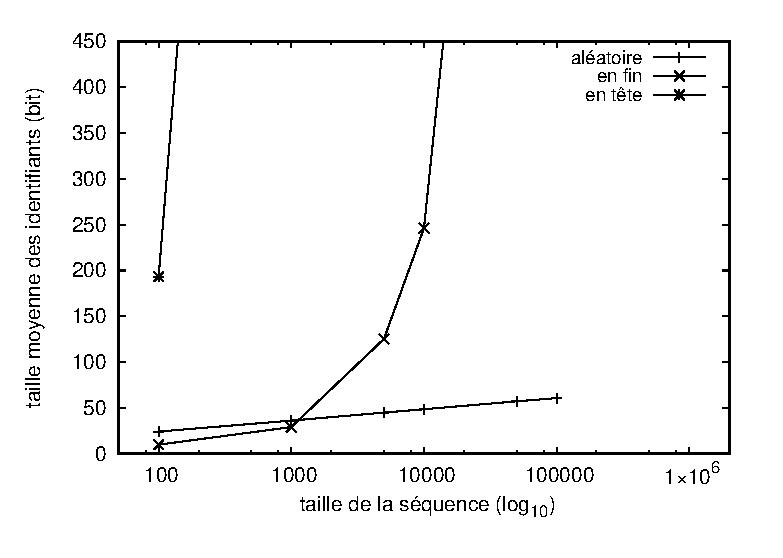
\includegraphics[width=.8\textwidth]{./img/lseq/logoot.eps}
  \caption{\label{fig:lseq:logoot}Stratégie d'allocation de référence adaptée à
    l'édition de gauche à droite utilisant un arbre d'arité maximum
    constante. Cette configuration correspond à Logoot.}
\end{figure}

% \begin{figure*}
%   \centering
%   \subfloat[Référentiel Logoot]
%   [\label{fig:lseq:logoot}Logoot comme stratégie d'allocation référentielle.]
%   {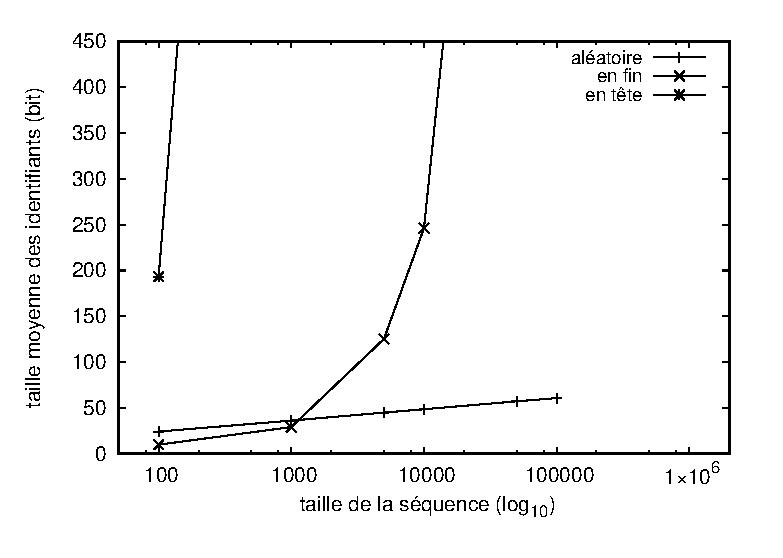
\includegraphics[width=0.48\textwidth]{./img/lseq/logoot.eps}}
%   \hspace{10pt}
%   \subfloat[Alternance de stratégies]
%   [\label{fig:lseq:robin}Alternance de stratégie d'allocation antagonistes.]
%   {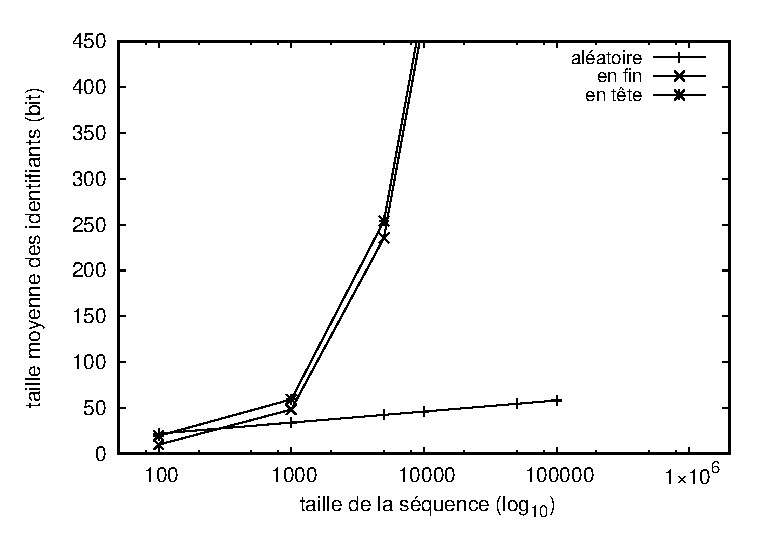
\includegraphics[width=0.48\textwidth]{./img/lseq/robin.eps}}
%   \caption{Résultat des expérimentations impliquant une structure d'arbre avec
%     arité constante.}
% \end{figure*}

\begin{asparadesc}
\item [Objectif:] Montrer que la stratégie impliquant la structure d'arbre dont
  l'arité est constante avec une stratégie adapté à l'édition monotone en fin
  possède une complexité spatiale linéaire lorsque l'édition est monotone,
  logarithmique lorsque l'édition est aléatoire.
\item [Description:] Les mesures concernent la taille moyenne (en bits) des
  chemins alloués pour les identifiants. Les mesures sont effectuées à 100,
  1000, 5000, 10000, 50000, 100000 insertions dans la séquence. Les chemins sont
  alloués dans un arbre dont l'arité est constante ($2^{10}$). La stratégie
  d'allocation examinée est adaptée à l'édition en fin. Ce système correspond à
  aux composants de Logoot.
\item [Résultat:] La figure~\ref{fig:lseq:logoot} présente le nombre d'insertions sur
  l'axe des abscisses (avec une échelle logarithmique en base décimale). L'axe
  des ordonnées correspondent à la taille moyenne des identifiants (en
  bits). Comme attendu, la taille moyenne des identifiants augmente lors de l'
  insertion d'éléments dans la séquence. Lors de l'édition aléatoire,
  l'augmentation de taille des identifiants est logarithmique. Lors de l'édition
  monotone, l'augmentation est linéaire. Toutefois, l'édition en tête est
  extrêmement coûteuse. L'édition en fin reste acceptable en comparaison de
  l'édition en tête, mais l'augmentation linéaire de la taille des identifiants 
  conduirait inéluctablement à un coûteux \emph{garbage collect}.
\item [Explication:] L'édition en tête et en fin ont tendance à déséquilibrer
  une branche de l'arbre stockant les identifiants. La stratégie d'allocation
  étant spécifiquement adapté à l'édition en fin, elle réserve des branches en
  fin d'arbre en allouant les branches les plus à gauche. Hélas, la même
  stratégie avec comportement d'édition en opposition conduit à une augmentation
  rapide de la profondeur de l'arbre. Dans le pire cas, la taille totale des
  identifiants est de complexité $O(nb_insert^2)$. Pour de similaires raisons,
  l'édition à des positions aléatoires conduit à une augmentation logarithmique
  car la structure d'arbre est équilibrée.
\end{asparadesc}

\ \\

\begin{figure}
  \centering
  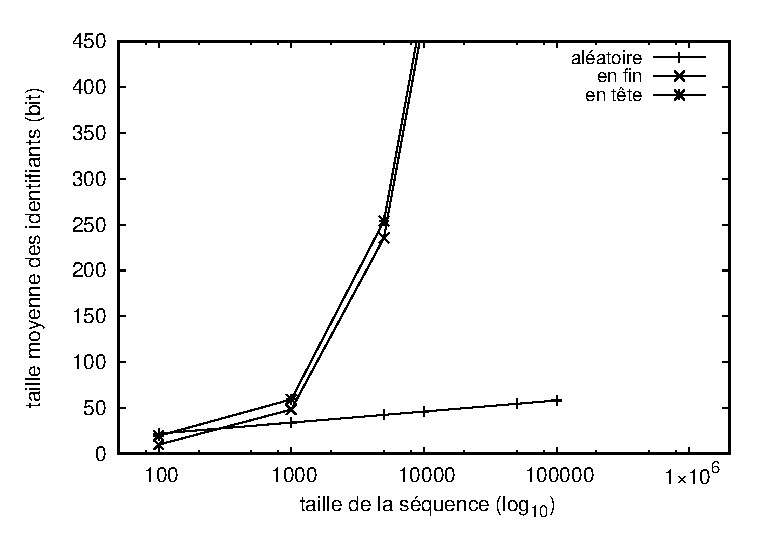
\includegraphics[width=.8\textwidth]{./img/lseq/robin.eps}
  \caption{\label{fig:lseq:robin}Stratégie d'allocation alternant deux
    sous-stratégies antagonistes utilisant un arbre d'arité maximum
    constante. L'une adaptée à l'édition de gauche à droite, l'autre adaptée à
    l'édition de droite à gauche.}
\end{figure}


\begin{asparadesc}
\item [Objectif:] Montrer que l'alternance des sous-stratégies d'allocation par
  profondeur équilibre la taille des identifiants alloués lors de l'édition
  monotone de droite à gauche et de gauche à droite. Cette alternance n'a aucun
  impact sur l'édition aléatoire.
\item [Description:] Les mesures concernent la taille moyenne (en bits) des
  chemins alloués pour les identifiants. Les mesures sont effectuées à 100,
  1000, 5000, 10000, 50000, et 100000 insertions. La stratégie d'allocation
  consiste à alterner les sous-stratégies d'allocations adaptées à l'édition
  monotone. Ainsi, si les profondeurs paires de l'arbre ont une sous-stratégie
  adaptée à l'édition de gauche à droite, les profondeurs impaires de l'arbre
  ont une sous-stratégie adaptée à l'édition de droite à gauche. Les chemins
  sont choisis dans un arbre dont l'arité maximum est constante et égale à
  $2^{10}$.
\item [Résultat:] La figure~\ref{fig:lseq:robin} présente les résultats de cette
  expérimentation. L'axe des abscisses représente le nombre d'insertions
  effectués dans la séquence sur une échelle logarithmique en base
  décimale. L'axe des ordonnées présente la taille binaire moyenne des chemins
  des identifiants. La figure~\ref{fig:lseq:robin} montre que pour les deux
  comportements d'édition, la forme de courbe est identique avec une
  augmentation linéaire en fonction du nombre insertions. La courbe
  correspondant à l'édition de gauche à droite est très légèrement meilleur. La
  taille des identifiants lors de l'édition aléatoire identique à celle de la
  figure~\ref{fig:lseq:logoot}. En d'autres termes, l'alternance de
  sous-stratégies n'améliore ni n'empire l'allocation d'identifiants lors de
  l'édition aléatoire.
\item [Explication:] En comparaison des résultats de la
  figure~\ref{fig:lseq:logoot}, la taille des identifiants lors de l'édition
  monotone est deux fois plus élevée. En effet, l'alternance de sous-stratégie
  évite le pire cas de la première expérimentation. Cette amélioration coûte un
  niveau de l'arbre tous les deux niveaux lorsque la sous-stratégie assignée à
  ce niveau est inadaptée. La complexité spatiale reste linéaire comparée au
  nombre d'insertions lors d'édition monotone. La complexité spatiale lors de
  l'édition monotone reste logarithmique car l'arbre représentant la séquence
  devient équilibré.
\end{asparadesc}

% \begin{figure*}
%   \centering
%   \subfloat[Augmentation de l'espace d'allocation]
%   [\label{fig:lseq:double}Augmentation de l'espace d'allocation en fonction de 
%   la profondeur de l'arbre.]
%   {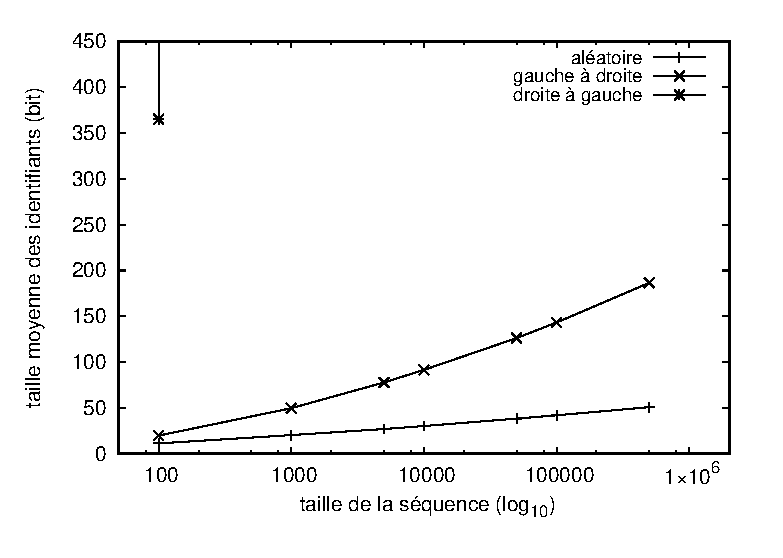
\includegraphics[width=0.48\textwidth]{./img/lseq/double.eps}}
%   \hspace{10pt}
%   \subfloat[Alternance et augmentation de l'espace d'allocation]
%   [\label{fig:lseq:lseq}\LSEQ comme combinaison de l'alternance et de l'augmentation.]
%   {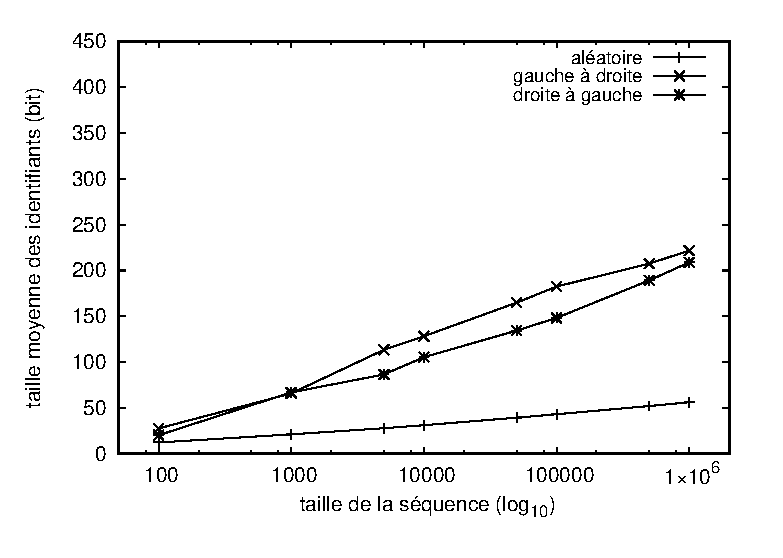
\includegraphics[width=0.48\textwidth]{./img/lseq/lseq.eps}}
%   \caption{Résultat des expérimentations impliquant une structure d'arbre exponentiel.}
% \end{figure*}

\begin{figure}
  \centering
  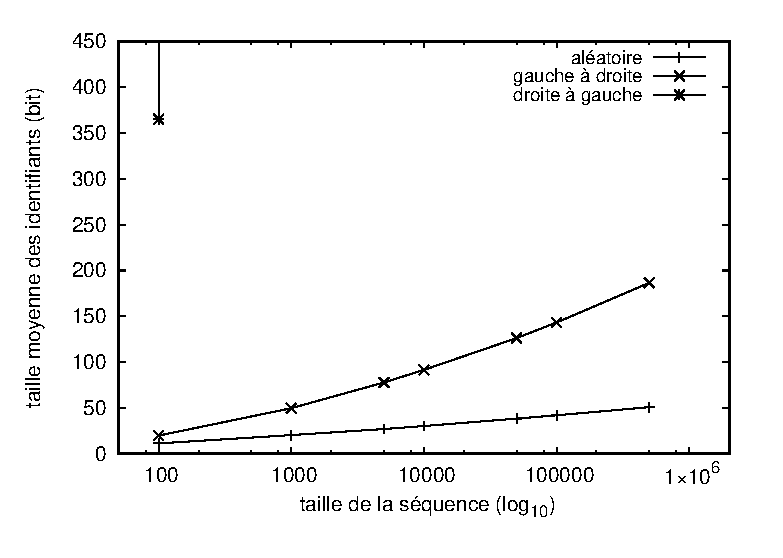
\includegraphics[width=.8\textwidth]{./img/lseq/double.eps}
  \caption{\label{fig:lseq:double}Stratégie d'allocation adaptée à l'édition de
    gauche à droite utilisant un arbre exponentiel.}
\end{figure}

\ \\

\begin{asparadesc}
\item [Objectif:] Montrer que l'utilisation d'un arbre exponentiel améliore la
  complexité spatiale des identifiants alloués lorsque le comportement d'édition
  est conforme à celui attendu. Montrer que cette amélioration implique une
  aggravation des identifiants alloués lors de l'édition pire cas.
\item [Description:] Les mesures concernent la taille moyenne (en bits) des
  chemins alloués pour les identifiants. Les mesures sont effectuées à 100,
  1000, 5000, 10000, 50000, 100000, et 500000 insertions. La stratégie
  d'allocation est adaptée à l'édition de gauche à droite. Les chemins sont
  choisis dans un arbre exponentiel dont l'arité maximum commence à $2^{5}$.
\item [Résultat:] La figure~\ref{fig:lseq:double} présente les résultats de
  cette expérimentation. L'axe des abscisses représente le nombre d'insertions
  effectués dans la séquence sur une échelle logarithmique en base
  décimale. L'axe des ordonnées présente la taille binaire moyenne des chemins
  des identifiants. Les résultats confirment les analyses en complexité de la
  section~\ref{sec:lseq:proposal}. Tout d'abord, lors de l'édition monotone de
  gauche à droite, la taille des identifiants augmente de manière
  polylogarithmique comparé au nombre d'insertions effectuées dans la séquence.
  Cette amélioration implique une dégradation de la complexité spatiale lors du
  pire comportement d'édition possible, ici, l'édition monotone de droite à
  gauche. Dans ce cas, la complexité spatiale est quadratique comparé au nombre
  d'insertions effectuées dans la séquence. Enfin, comme les expérimentations
  précédentes, la complexité de l'édition aléatoire est
  logarithmique. Toutefois, les résultats de l'édition aléatoire sont meilleurs
  en valeur absolue.
\item [Explications:] La stratégie d'allocation employée est adaptée à l'édition
  de gauche à droite. Ainsi, lorsque le comportement d'édition suit cette
  hypothèse, l'une des branches de l'arbre exponentiel se remplit efficacement.
  Plus la profondeur de l'arbre grandit, plus les éléments peuvent accueillir
  d'éléments en tant que fils. Cette stratégie suppose qu'une augmentation de la
  profondeur reflète un document grandissant. Malheureusement, lorsque
  l'augmentation est due à un comportement d'édition non prévu, l'allocation
  perd d'autant plus d'espace. D'où l'augmentation quadratique lors du pire cas
  d'édition. De façon similaire aux expérimentations précédentes, l'édition
  aléatoire résulte en un arbre équilibré, d'où l'augmentation logarithmique des
  identifiants. La taille de départ de l'arbre exponentiel étant plus faible
  ($2^{5}$ contre $2^{10}$), la représentation binaire des identifiants est
  meilleure en valeur absolue.
\end{asparadesc}

\begin{figure}
  \centering
  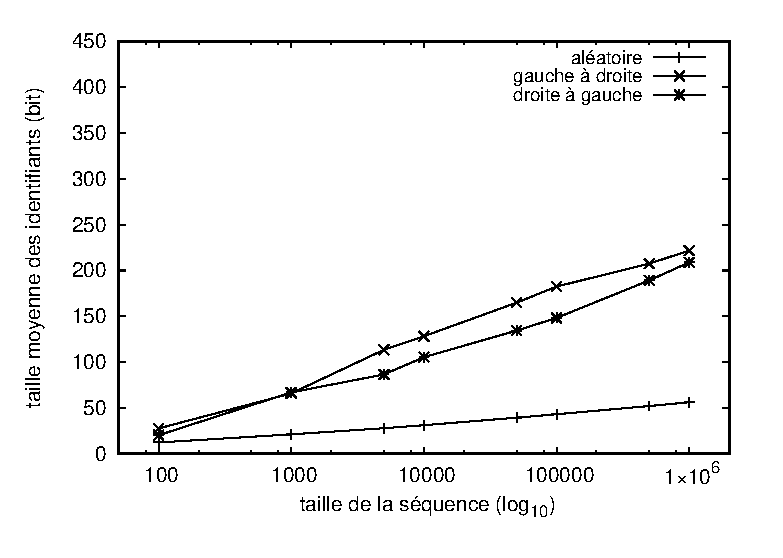
\includegraphics[width=.8\textwidth]{./img/lseq/lseq.eps}
  \caption{\label{fig:lseq:lseq}Stratégie d'allocation utilisant deux
    sous-stratégies antagonistes adaptées aux éditions monotones et utilisant un
    arbre exponentiel. Cette configuration correspond à \LSEQ.}
\end{figure}

\ \\

\begin{asparadesc}
\item [Objectif:] Montrer que la stratégie d'allocation \LSEQ comme composition
  de l'alternance de sous-stratégies antagonistes adaptées à l'édition monotone
  avec un arbre exponentiel permet de remédier au pire cas des précédentes
  expérimentations tout obtenant une complexité polylogarithmique à ces types
  d'édition.
\item [Description:] Les mesures concernent la taille moyenne (en bits) des
  chemins alloués pour les identifiants. Les mesures sont effectuées à 100,
  1000, 5000, 10000, 50000, 100000, 500000, et 1000000 insertions. La stratégie
  d'allocation est \LSEQ. Ainsi, deux sous-stratégies d'allocations adaptés à
  l'édition monotone sont assignées successivement à chaque niveau de l'arbre
  exponentiel. Ce dernier possède une arité maximum de départ de $2^5$.
\item [Résultat:] La figure~\ref{fig:lseq:lseq} présente les résultats de cette
  expérimentation. L'axe des abscisses représente le nombre d'insertions
  effectués dans la séquence sur une échelle logarithmique en base
  décimale. L'axe des ordonnées présente la taille binaire moyenne des chemins
  des identifiants. Comme attendu, les deux types d'édition monotone possède le
  même profil, à savoir, une augmentation polylogarithmique de la taille des
  identifiants comparé au nombre d'insertions effectuées dans la séquence. La
  taille moyenne des identifiants alloués par \LSEQ lors de l'édition aléatoire
  augmente logarithmiquement.
\item [Explication:] \LSEQ se comporte bien dans les deux types d'édition
  monotone car lorsque un niveau de l'arbre exponentiel est perdu, le niveau
  qui suit en compense les pertes.
\end{asparadesc}

\subsubsection{Simulations avec concurrence}

\begin{figure*}
  \centering
  \subfloat[Utilisateur unique]
  [\label{fig:one}Augmentation de l'espace d'allocation en fonction de 
  la profondeur de l'arbre.]
  {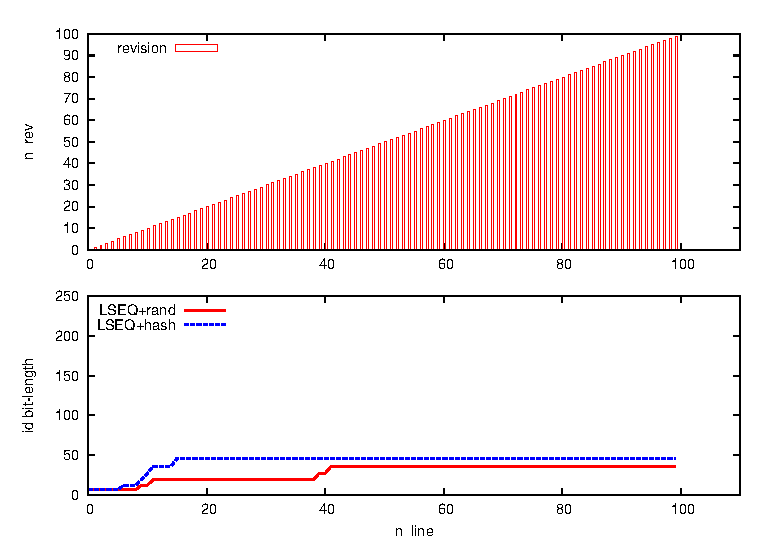
\includegraphics[width=0.48\textwidth]{./img/lseq/oneuser.eps}}
  \hspace{10pt}
  \subfloat[Alternance et augmentation de l'espace d'allocation]
  [\label{fig:ten}\LSEQ comme combinaison de l'alternance et de l'augmentation.]
  {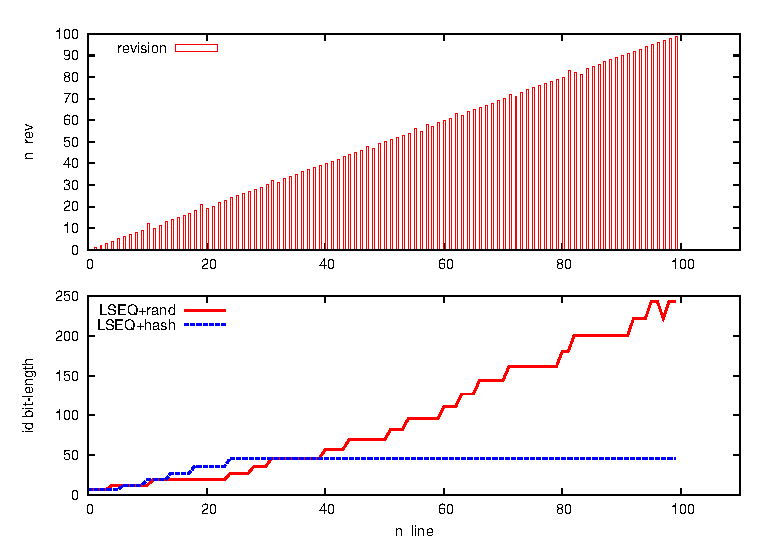
\includegraphics[width=0.48\textwidth]{./img/lseq/tenusers.eps}}
  \caption{Spectre de document artificiel générés par insertion répétée de caractère
  en fin.}
\end{figure*}

\begin{asparadesc}
\item [Objectif:] \TODO{À refaire!} Montrer l'importance d'une fonction
  d'assignation de sous-stratégie commune à tous les possesseurs de la séquence
  répliquée.
\item [Description:]
\item [Résultat:]
\item [Explication:]
\end{asparadesc}

\subsubsection{Simulations sur traces Wikipedia}

\begin{figure*}
  \centering
  \subfloat[Comportement d'édition attendu]
  [\label{fig:compliant}Le comportement d'édition correspond aux attentes
  de la stratégie d'allocation]
  {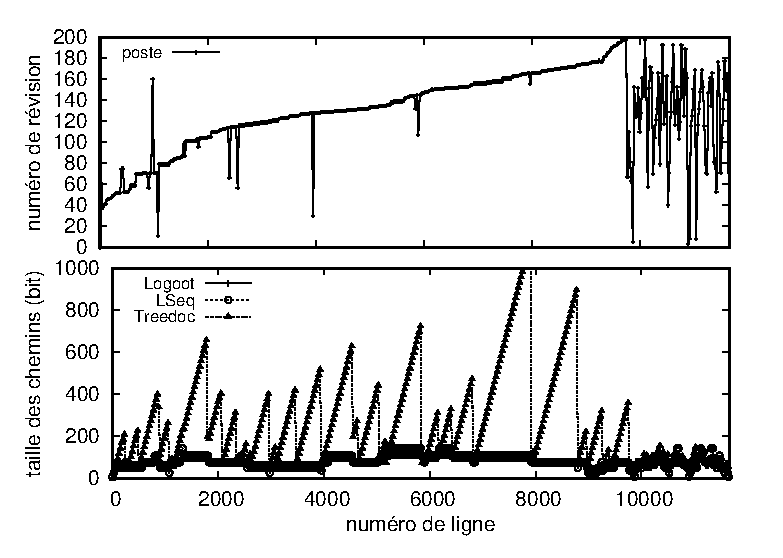
\includegraphics[width=0.48\textwidth]{./img/lseq/poste.eps}}
  \hspace{10pt}
  \subfloat[Comportement d'édition inattendu]
  [\label{fig:motivating}Le comportement d'édition va à l'encontre des attentes
  de la stratégie d'allocation]
  {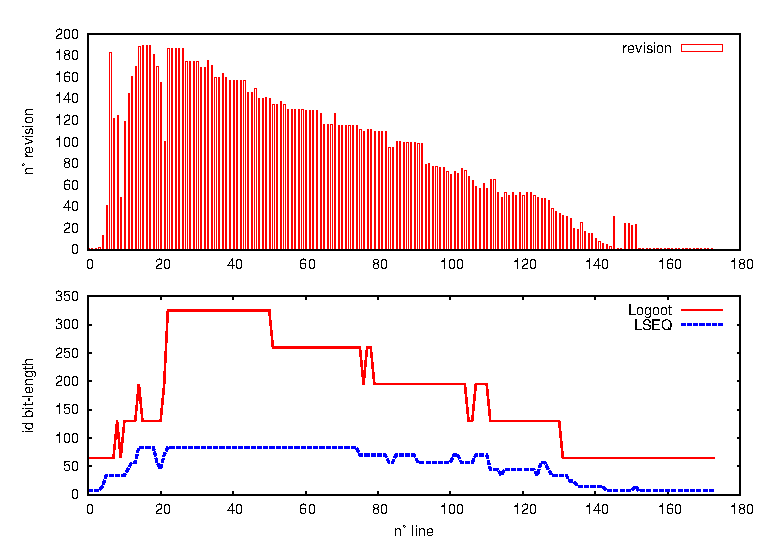
\includegraphics[width=0.48\textwidth]{./img/lseq/didyouknow.eps}}
  \caption{\label{fig:allocation}Spectre de document Wikipedia sous différent
    comportements d'édition antagonistes. La figure du haut représente la
    révision à laquelle la ligne a été inséré, i.e., sa date de naissance.  La
    figure du bas représente la taille de l'identifiant associé à chaque ligne.}
\end{figure*}

%%% Local Variables:
%%% mode: latex
%%% TeX-master: "../../paper"
%%% End:
